\documentclass{article}


% Language setting
% Replace `english' with e.g. `spanish' to change the document language
\usepackage[english]{babel}
% Set page size and margins
% Replace `letterpaper' with `a4paper' for UK/EU standard size
\usepackage[letterpaper,top=2cm,bottom=2cm,left=3cm,right=3cm,marginparwidth=1.75cm]{geometry}
% Useful packages
\usepackage{amsmath}
\usepackage{subcaption}
\usepackage{graphicx}
\usepackage[colorlinks=false, allcolors=blue]{hyperref}
\usepackage{booktabs}

\title{Exploring Scope of Using Multi-Agent Reinforcement Learning Systems for Efficient Warehouse Management with Robots}
\author{Ashish Rana, 1822317 \\
        ashish.rana@students.uni-mannheim.de}


\begin{document}
\maketitle
\tableofcontents % table of content
\listoftables % list of table added
\newpage


\begin{abstract}


In manufacturing, warehouse management is one of the laborious tasks especially in large scale warehouses for companies such as Amazon and Alibaba.
Additionally, for optimization the moving goods and packages task is rapidly going through digital transformation by using mobile robots to build automated warehouses.
This technical problem of Multi-agent Pickup and Delivery (MAPD) requires the system to assign tasks for agents and then generate collision-free paths.
The more traditional optimization based approaches solve this problem by using different search and collision strategies.
The results from these studies, even though highly optimized, require large domain specific engineering efforts governed by warehouse specifications.
Whereas, modern Multi-agent Reinforcement Learning Systems (MARLS) handles this two-step task with more flexibility by using approaches like, reward shaping, and hierarchical learning etc.
In our study we qualitatively and quantitatively compare these approaches and address their corresponding advantages and limitations in detail.
Also, the related code repository implementation and experimentation is present at \href{https://github.com/ashishrana160796/analyzing-cooperative-marls}{github.com/ashishrana160796/analyzing-cooperative-marls}.


\end{abstract}


\section{Introduction}


% introduction
% general introduction: warehouse management general problem, general description of the problem
% heuristic work: prior heuristic work for the problem, relevant studies and findings, limitations
% reinforcement learning: advantages of reinforcement learning work, reinforcement learning formulation
% our contribution: baseline insights from heuristic studies, multi-agent setting and comparison with heurisitic approaches
% The sections present in this literature review of marls for warehouse management
In automated warehouse management systems, ideally a team of robots works together to fulfill customer orders.
This team of robots unlike humans can work tirelessly and increase throughput manifolds for any warehouse management organization.
Coordinating robots in such a large system requires multiple components to work together like assigning management jobs to robots, finding optimal collision free paths, and infrastructure maintenance and upgradation etc.
This complete task problem has been formally studied in the past as separate Multi-robot task assignment (TA) and Multi-agent Path Finding (MAPF) problems \cite{korsah2013comprehensive, stern2019multi}.
But, these heuristic methods require significant engineering efforts and constant fine-tuning based on changing warehouse configurations and customer demand distribution.
Additionally, approaches only targeting fully automated robotic solutions lack practicality in deployment considering high maintenance, unexpected downtime possibilities, and discarding already existing mature infrastructure involving humans.
Considering the above described two major issues, in this manuscript we explore two MARLS experiments which attempt to introduce flexibility in operations, and utilization of existing warehouse management infrastructure for the warehouse management task.


In this manuscript, we first discuss and elaborate some prior concepts for the automated warehouse management problem, and reinforcement learning terminologies in multiple agent scenarios.
Second, we discuss experimentation and results for two MARLS studies, where the first study uses reward shaping to tackle sparsity problems in multi-agent warehouse settings.
The second study focuses on developing a practical and scalable solution with hierarchical RL to benchmark its proposed MARL performance against the heuristic approaches.
Finally, we conclude our exploration study and practically quantify the MARL application performance with small experimentation \footnote{Experimentation code available at the repository \href{https://github.com/ashishrana160796/analyzing-cooperative-marls}{github.com/ashishrana160796/analyzing-cooperative-marls}}.


\section{Related Work}


The MAPF problem is NP-hard to solve optimally where quality of solution of solution in makespan \textit{(maximum of arrival times of all agents at goal locations)} or flowtime \textit{(summation of arrival times of all agents at goal locations)}.
Previously, studies have attempted to solve the warehouse management problem, where TA and MAPF are either solved separately or in a combined manner \cite{korsah2013comprehensive}.
And, MAPF problem also has been studied in two settings, where either the whole MAPF problem is solved or it is broken into smaller MAPF sub-problems for saving computations \cite{stern2019multi}.
Integrated TA and MAPF is also explored as an improved alternative where task assignment choices are calculated with real delivery costs instead of lower-bound estimates \cite{chen2021integrated}.
As an improvement for MAPF subtask the corresponding study also uses marginal-cost assignment heuristic and large neighborhood search based meta-heuristic strategy for finding optimal paths.
Further, it is argued that MAPF independent of TA is a better alternative for building a more generalizable collision-free path finding system \cite{li2021lifelong}.
Where, rolling horizon windowed MAPF solvers using traditional search algorithms for resolving collisions have shown better results.
The modularity with different components involved adds complexity to the pipeline, and makes the performance of approach highly correlated with the design choices.
Below, we further discuss different automated warehouse management paradigms, and relevant background for MARLS which can serve as an end-to-end alternative.


\subsection{Practical Automated Warehouse Management Background} \label{warehouse-problem-background}


The order-picking task essentially consists of retrieving order items and delivering to target location, it generally accounts for 55 \% of operational cost for warehouses \cite{drury1988towards}.
Automation systems like Dematic Multishuttle1, Autostore2, and KIVA use the \textit{pick-to-picker} paradigm where autonomous systems move items to pickers for dispatch to customers \cite{wurman2008coordinating}.
These systems are more costlier in warehouses with varying scale and flexible demands in comparison to the \textit{picker-to-pick} paradigm, which accounts for 80\% of warehouses in Western Europe \cite{de2007design}.
In this paradigm the picker robots go to the item locations to directly retrieve and dispatch the item.
More practical automated warehouse management studies formulate their solutions around these paradigms for better benchmarking with existing solutions.


% summarize three sections from the related work section
% elaborate with 2 seperate paragraphs for the 2 heuristic based approaches, add some diagrams
% FM, PDM explain in detail additionally (3.2), and also highlight associated challenges (3.3)


There are several key challenges for managing warehouses realistically at large scale for improving key performance indicators like, pick rate, idle time, and distance traveled.
For \textit{picker-to-pick} paradigm heuristic approaches like \textit{Follow Me} (FM), and \textit{Pick, Don’t Move} (PDM) have shown promising results.
In FM, a cluster of AGVs are assigned to each picker to follow, and a traveling salesman problem (TSP) solution for all the AGVs to determine order fulfillment sequence.
It improves the efficiency by minimizing idle time for pickers, but might increase their travel time and distance leading towards efficiency and energy consumption trade-off.
Whereas in PDM, pickers are allocated to zones in the warehouse, and AGVs are permitted to travel throughout the warehouse.
The AGVs are picked by pickers based on the AGV and its target location’s proximity, where AGV travels through the order list using the TSP solution.
Pickers movement is limited to zones but requires timely movement for loading and unloading AGVs.
This approach minimizes the travel distance for pickers but might lead to under-utilization of pickers.


The heuristic strategies in general require repeated fine-tuning based on different use-cases.
Depending on customer and context we might have to change many factors like, item clustering design, order priority mechanism, demand and supply logistics, labor and automation workforce conditions, and regulatory factors.
This is an iterative and resource heavy process involving multi-party interactions leading to regular additional engineering effort for obtaining the most optimized solution.
This suboptimal behavior issue transpires multi-faceted solutions exploring automated agent-policy solutions which address scalability and productionisation concerns.


Practically relevant solutions for the automated warehouse management problem address three main aspects, namely: i) pipeline scalability, ii) solution environment, and iii) productionisation.
The scalable solutions is expected to handle magnitude and complexity of different dimensions of problems like, number of item locations \textit{$|$L$|$}, order distribution denoted by \textit{Z}, number of vehicle and picker workers represented by \textit{$|$V$|$} + \textit{$|$P$|$} respectively.
With increasing complexity handling large numbers of agents centrally becomes harder as joint action space grows exponentially which makes decentralized individual executor agents a preferred choice in MARLS.
MARL algorithm requires large interaction with the environment for learning, and initially learnt joint policies might be highly suboptimal for given warehouse configuration \cite{papoudakis2020benchmarking}.
Therefore, a high performance simulation platform is important for the development and testing pipeline.
Finally, a practical system should exist in an ecosystem of integrable tools either on-premise or on cloud which can help execute the code in distributed manner, and debug model performance after observing sub-optimal behavior.


\subsection{Reinforcement Learning Problem Background} \label{rl-problem-background}


RL tasks can be classified into model-free and model-based modeling types, where in model-free learning agents get rewards with policy actions.
But, in model-based learning agents already know the reward and probability transition functions i.e. internal environmental models.
For warehouse management problems it is better to opt for model-free learning because internal environment dynamics might vary based on scenarios, and modeling such dynamics to great details might be computationally unnecessary as well.
Both value and policy based approximation methods have shown promising results for multiple RL tasks.
But, architectures using both these approximation approaches, like actor-critic models, are more capable of handling complex scenarios \cite{sutton2018reinforcement}.
For multi-agent systems the Markovian assumption does not hold, there the Markovian Decision Process (MDP) modeling of the RL problem is dropped. And, the stochastic game setting is chosen where a combination of agent actions determines the next state and reward with partially observable environment characteristic \cite{hansen2004dynamic}.


MARL systems can be divided into three types based on task characteristics and the agent relationships.
First, cooperative type where agents work together to achieve a common goal having a common reward model.
And second it's opposite a competitive setting where the reward system is modeled as a zero-sum game.
The third type is the mixed one which is less restrictive, the warehouse management problem can be modeled as cooperative or mixed scenario MARL depending on the use-case.
Additionally, for learning and execution the MARLS can again be divided into three types, namely: i) Centralized Training Centralized Execution (CTCE), ii) Centralized Training Decentralized Execution (CTDE), iii) Distributed Training Decentralized Execution (DTDE).
In CTCE, centralized policy is learnt and used by the agents, during training agents influence each other which might make learning inefficient.
The vice-versa is applicable for DTDE which involves independent learners, and both these approaches fail to scale because of the learning task complexity.
Finally, in CTDE agents share the same learning model and experience with common goals but agents perceive their interactions differently, resulting in different behavior.
For warehouse management problems in simpler scenarios CTCE, and for scenarios requiring scalability CTDE can be used, as both provide simplicity and efficiency for respective modeling requirements \cite{wen2021dtde}.


In simpler scenarios, for value based methods Deep Q-Networks (DQN) learns non-linear optimal action-value function following the Bellman Equation.
Further, Double Deep Q-Networks (DDQN) select action from current Q-Network and evaluate it using the old Q-Network to avoid instability in Q-Values while learning.
Further, Independent Q-Learning (IQL) maximizes joint rewards by observing the local information.
Where individual agents execute the Q-Learning algorithm and calculate its own loss based on local information \cite{sutton2018reinforcement, wen2021dtde}.
For warehouse management and other RL tasks, defining different reward distributions with changing configurations and use-case can be very hard.
Further, not assigning dense reward signals might create sparsity problems as well.
For the sparse reward problem, several approach alternatives have been explored, like reward shaping, transfer learning, imitation learning, curriculum learning, curiosity-driven learning, and hierarchical RL (RL) \cite{huang2020action}.


\section{Multi-Agent Reinforcement Learning Approaches}


In below subsections we analyze two different MARLS studies for automated warehouse management which analyze the warehouse package delivery problem at different abstraction levels.
The first study presents a completely automated warehouse system with only robots, and handles theoretically novel sparse reward problems to improve existing RL algorithms \cite{lee2022marl}.
Whereas, the second study envisions highly practical mobile robot and human picker based hybrid systems at more realistic scales \cite{krnjaic2022scalable}.
This study further compares its findings and results with existing heuristic benchmarks to accurately quantify its performance in comparison to existing successful approaches.


\subsection{Reward Models on Segmented Actions for Agents}


Modeling automated warehouse management as MARLS gives the solution relatively better flexibility and adaptability in comparison to traditional heuristic based approaches.
But, with MARLS systems their own set of challenges needs to be resolved, like defining appropriate reward schemes.
Also, reward engineering is especially challenging when for MARL systems and might lead to unexpected consequences if appropriate domain knowledge is missing \cite{cabi2019scaling}.
Qualitatively for this modeling only after a large sequence of actions within a complex delivery path a reward is assigned to the agents leading to sparse reward problem.
The experimentation study elaborated in this section resolves this issue by using a separate dual reward system during the initial and ending stages of the package delivery \cite{lee2022marl}.
This newly defined reward system eventually helps in learning the package delivery task in a more stable manner for multiple robots in the warehouse environment.


\begin{figure}
\centering
\begin{subfigure}[b]{0.4\textwidth}
   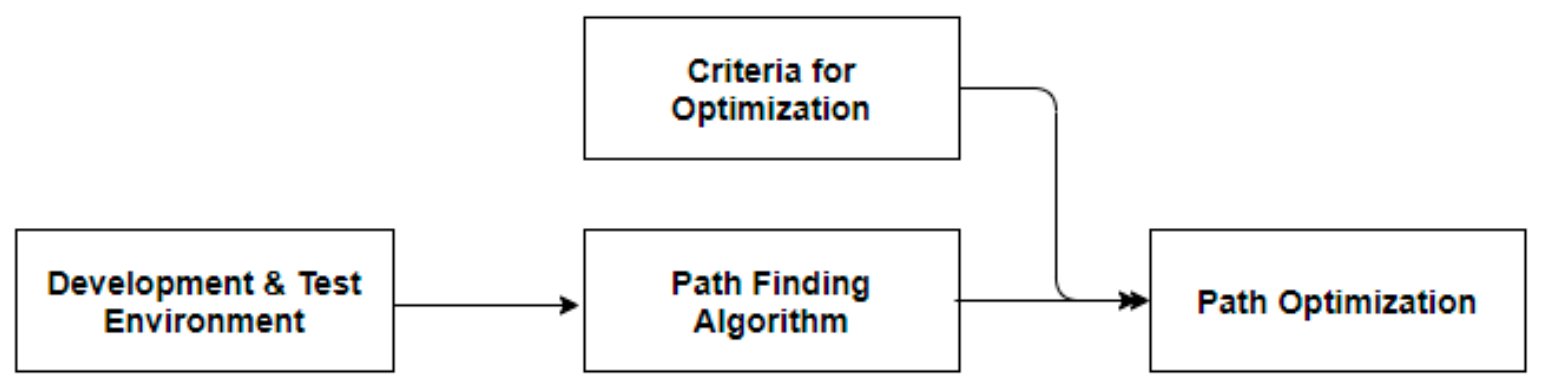
\includegraphics[width=1\linewidth]{path-planning-problem.png}
   \caption{Path planning steps for optimization.}
   \label{fig:abstract-opt-prob} 
\end{subfigure}

\begin{subfigure}[b]{0.4\textwidth}
   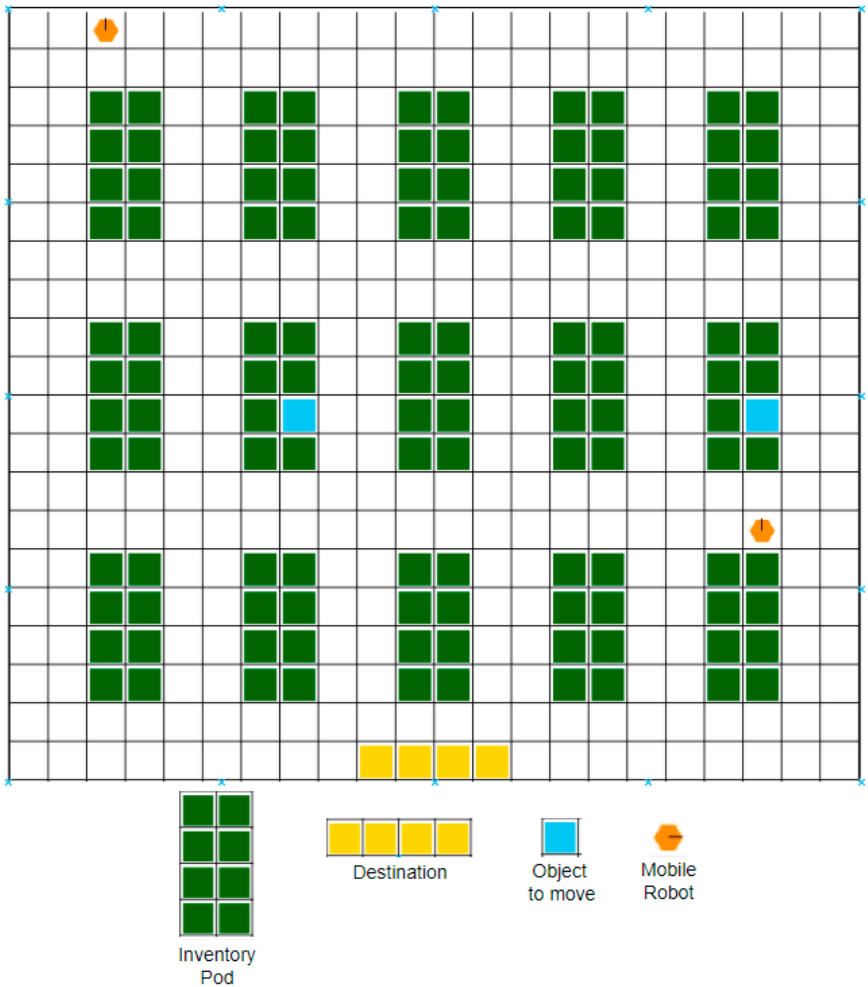
\includegraphics[width=1\linewidth]{warehouse-layout.png}
   \caption{Example of warehouse environment layout.}
   \label{fig:warehouse-layout}
\end{subfigure}

\caption[Path planning on warehouse layout]{(a) Different modules in package delivery problem for the automated warehouse layout. (b) Warehouse grid layout with green inventory pods from which packages are delivered to yellow workstations. \textit{(Image Credit: Lee et al.)}}
\end{figure}


The path planning task for delivering packages in the automated warehouse management problem comprises components like, path finding algorithm, path optimization, and optimization criteria for given development and testing environment, as shown in Figure \ref{fig:abstract-opt-prob}.
The reinforcement learning approach for multiple agents abstracts away these heuristic specific components and attempts to model the whole process as an end-to-end task. 
Also, for the warehouse environment the reinforcement learning problem is developed in an abstracted and simplistic sparse simulation environment.
The RWARE environment used in the dual reward system study simulates package shelf pick-ups by robots, workstation drops, and empty shelf returns in the specified layout in Figure \ref{fig:warehouse-layout}.
In this environment, the mobile robot first finds and reaches the object location to pick up the object and place it on a transportation tray.
After that, the robot places the package on the workstation and delivers the transportation tray back to initial position.
For the experimentation the final workstation destination is fixed but robot starting and initial package locations are changed randomly.


% https://www.mdpi.com/2076-3417/12/9/4703
% https://www.researchgate.net/publication/360461110_MARL-Based_Dual_Reward_Model_on_Segmented_Actions_for_Multiple_Mobile_Robots_in_Automated_Warehouse_Environment


% reward model -> 3.2.3 dual reward segmentation model describe, 4.3 section explain the dual reward algorithm
% training for model -> DQN, DDQN, IQL algorithm
% elaborate the plot findings for different plots


% 4 para: complete system and reward model theory, experiment setup & algorithm, 2 paragraphs of results
% 3 figs: 1 system diagram, 1 reward model example, 1 figures for plots
\begin{figure}[h]
    \centering
    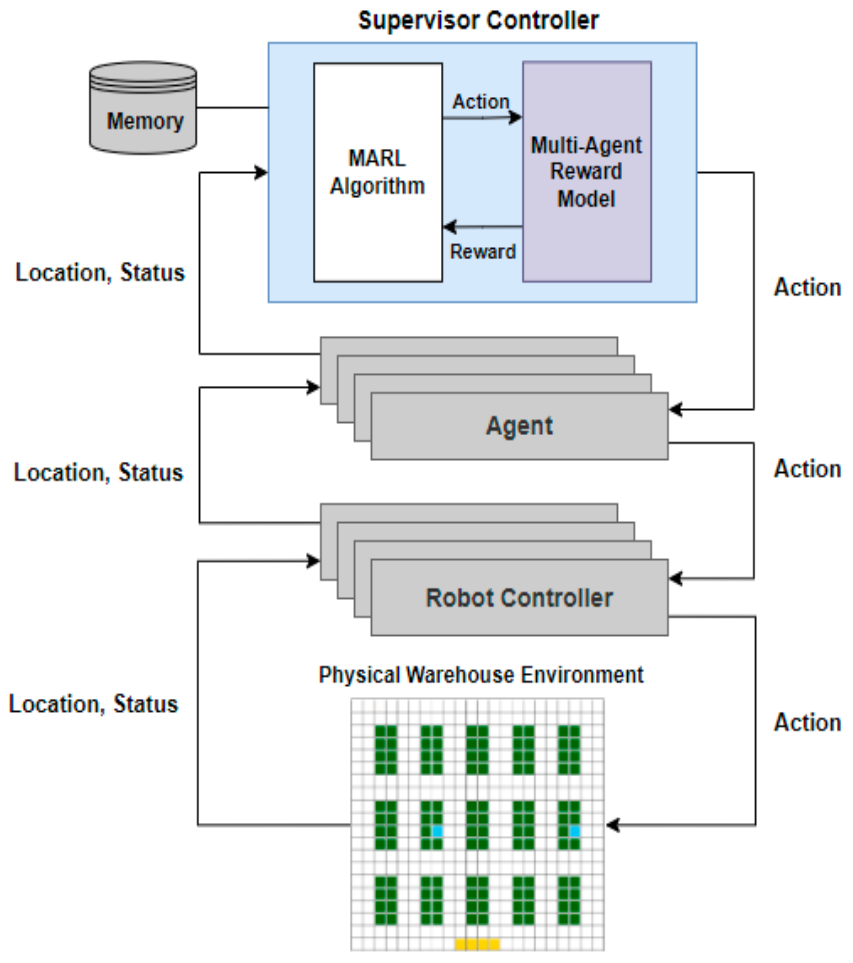
\includegraphics[width=0.375\textwidth]{reward-shaping-pipeline.png}
    \caption{MARL mobile robot framework pipeline for warehouse management. \textit{(Image Credit: Lee et al.)}}
    \label{fig:reward-shaping-pipeline}
\end{figure}


The Figure \ref{fig:reward-shaping-pipeline} functionally describes the MARLS pipeline and the incorporation of the dual segmented reward model into that pipeline.
The dual segmented reward model applies specific rewards for partial actions instead of full actions, where a full action is a union of sequence of partial actions.
A partial action functionally defines a subtask only, like move to pick up an object, move to destination with object, return empty tray back etc.
Whereas a full action comprises all the partial actions needed to deliver the object, and return the empty tray until the whole task is completed.
For distinguishing goal achieving agents, cooperative and competitive relationships are also mixed for agents.
Here, a relatively larger reward is assigned to agents that achieve the goal in comparison to agents that didn’t complete the task.
The dual segmented reward model study divides the reward signal of full actions defined functionally into distributed dense rewards over partial actions.
Previously, studies have shown effectiveness of this approach for tasks like dexterous manipulation, and path finding \cite{gudimella2017deep, sartoretti2019primal}.



\begin{figure}[!tbp]
  \centering
  \subfloat[First reward model for initial stages.]{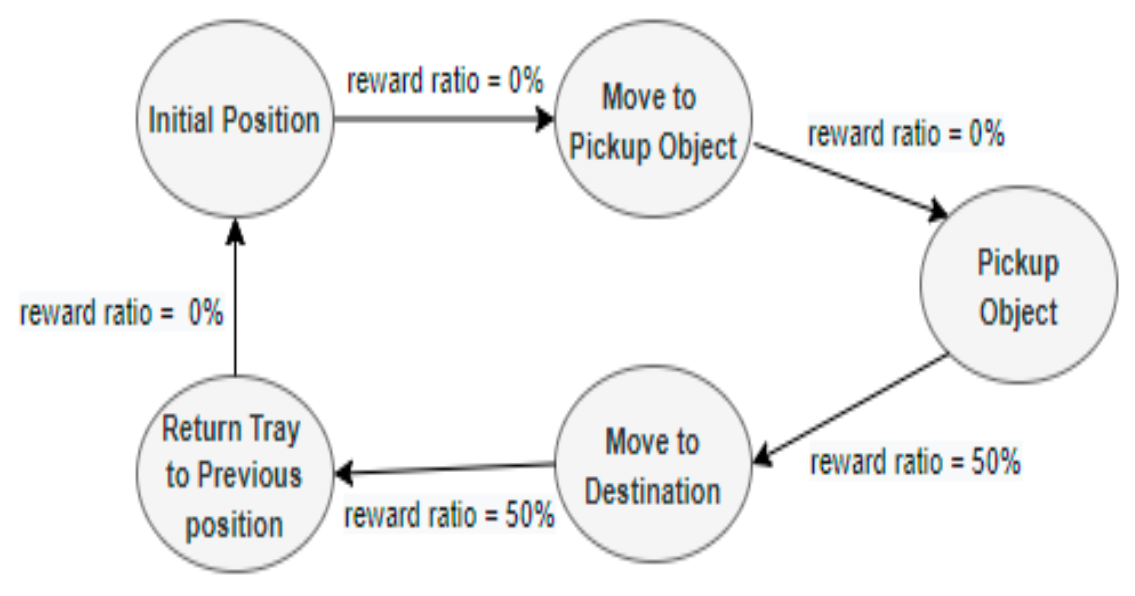
\includegraphics[width=0.375\textwidth]{reward-model-a.png}\label{fig:reward-model-a}}
  \hfill
  \subfloat[Second reward model for final stages.]{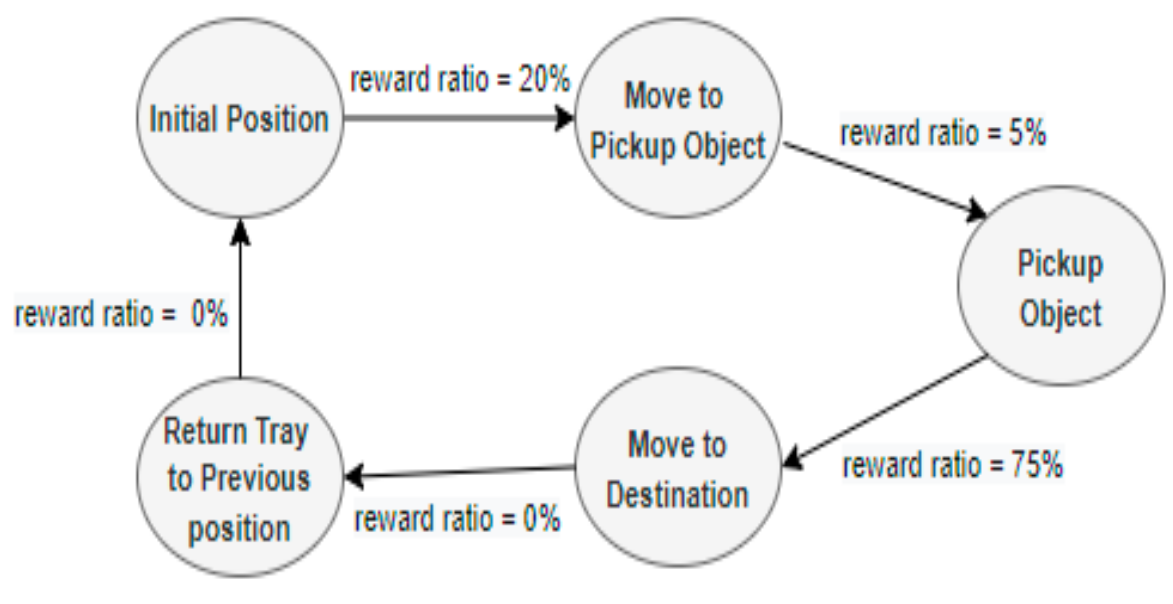
\includegraphics[width=0.375\textwidth]{reward-model-b.png}\label{fig:reward-model-b}}
  \caption{Segmented reward models assigning rewards for different subtask stages for removing sparsity problem meaningfully. \textit{(Image Credit: Lee et al.)}}
\end{figure}


\subsubsection{Experiments and Results}


By exploiting task specific domain knowledge the handcrafted dual segmentation model assigns rewards differently with two reward schemes during initial and later stages of model training.
In Figure \ref{fig:reward-model-a} representing the first reward model, in beginning learning stages the initial partial actions are rewarded with higher rewards.
For later learning stages the second reward model is utilized which encourages the task completion, refer Figure \ref{fig:reward-model-b}.
Additionally, for more stabilized learning a low learning rate of 0.00008, discount factor of 0.99, and reward decay rate of 0.99 with increasing episode count was also used.
For experimentation, the environment scale includes 2 agents and 15 inventory pods where MARLS with DQN-based, and DDQN-based IQL algorithm models were trained.
In IQL algorithms each agent maintains its own Q-values where it makes local information based belief updates, and assumes other agents are part of the environment.
This approximation essentially results in the loss of convergence guarantee of the Q-Learning algorithm as other agents introduce non-stationarity in the environment.


\begin{figure}[h]
    \centering
    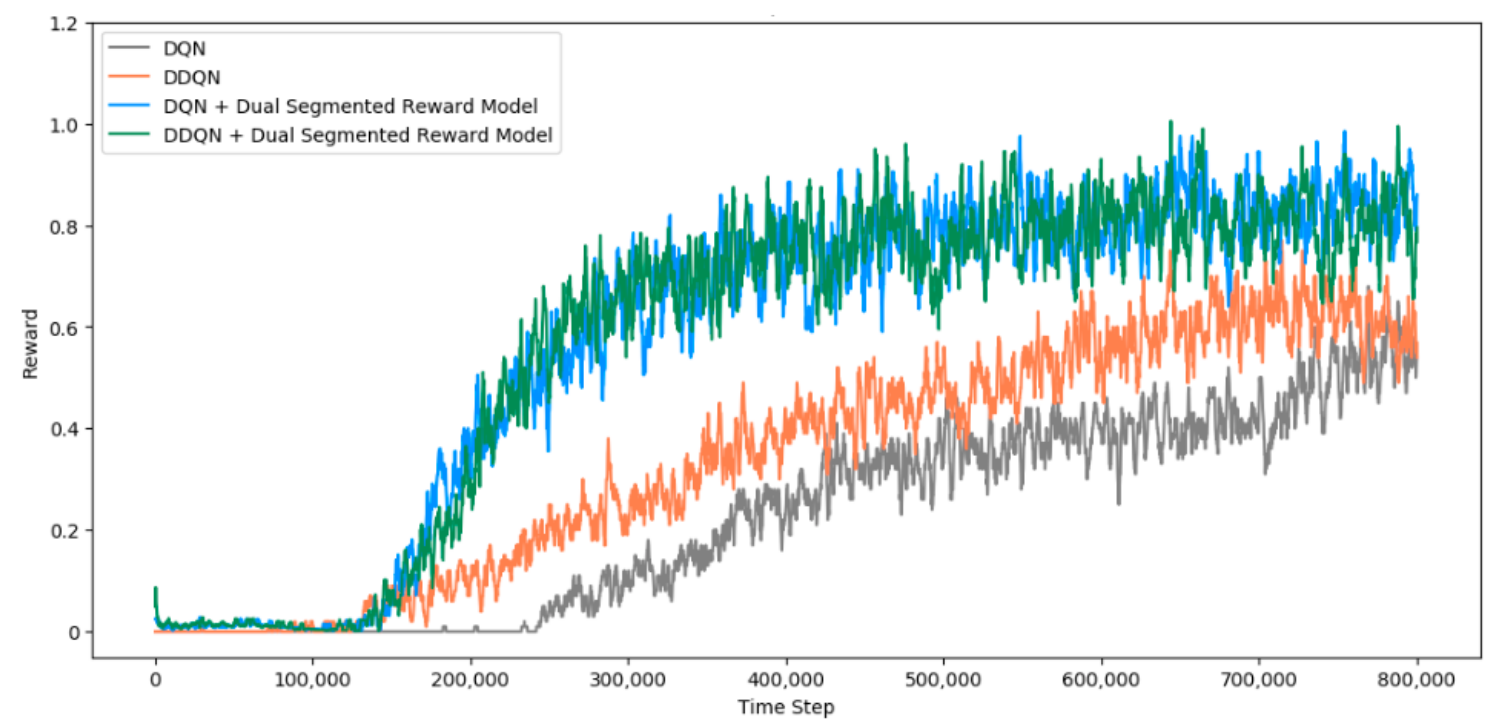
\includegraphics[width=0.6\textwidth]{reward-shaping-result.png}
    \caption{Reward accumulation analysis summary for DQN, DDQN, DQN with segmented reward model, and DDQN with segmented reward model. \textit{(Image Credit: Lee et al.)}}
    \label{fig:reward-shaping-result}
\end{figure}


In results, for vanilla DQN and DDQN the instability is quite high in comparison to their dual segmented reward shaped trained counterpart agent systems which produced less convergence variance.
Additionally, from Figure \ref{fig:reward-shaping-result} it is also observed that the dual segmented reward shaped models converged faster in comparison to models that weren’t reward shaped.
Further, across multiple runs even at earlier stages the dual segmented reward shaped models demonstrate accumulation of positive reward signal highlighting higher initial exploration tendencies.
Additionally, from the convergence curves we also observe that both DQN and DDQN models have similar and better performance in comparison to their vanilla counterparts where DDQN performs relatively better than DQN.
Further, as a limitation the correlation of this highly use-case specific reward system with better performance and environment simplicity was also highlighted.


\subsection{Scalable Hierarchical Learning for Agents}


This scalable MARLS study with automated guided vehicles (AGVs) and human co-workers focuses on a more practical collaboration based scenario for managing warehouse logistics.
This study specifically focuses on maximizing the order-lines \textit{(order comprises several order-lines)} per hour.
This metric in turn also affects average distance traveled and idle time for AGV and human co-worker agents.
This study considers breaking down the complex action space by incorporating multi-layer hierarchy in Shared Experience Actor-Critic (SEAC) learning architecture i.e. analyzing decomposed action space via Hierarchical Shared Experience Network Actor-Critic (HSNAC) to observe performance gains.
Also, Figure \ref{fig:scale-learn-pipeline} highlights the solution pipeline where the MARL algorithm runs on the AI controller with on-premise deployment for lowering the downtime.
The commands are transferred to AGVs via vehicle management system, and to human workers via a mobile device through an independent on-premise communication system.


\begin{figure}[h]
    \centering
    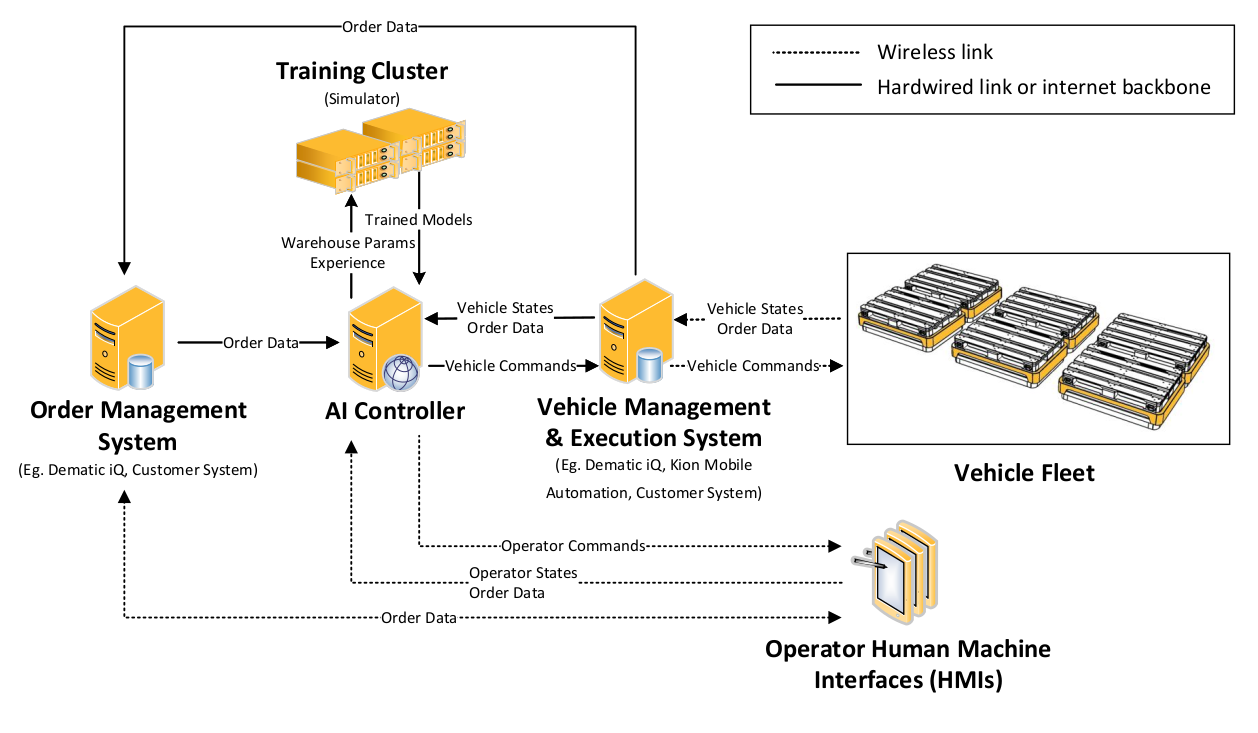
\includegraphics[width=0.75\textwidth]{scalable-rl-learning-example.png}
    \caption{System pipeline for the proposed scalable MARL solution. \textit{(Image Credit: Krnjaic et al.)}}
    \label{fig:scale-learn-pipeline}
\end{figure}


% discussion of paradigms of order picking
% advantages of building human-agv mixed system for package delivery
% https://sites.google.com/view/scalablemarlwarehouse/


The warehouse management problem previously was solved with three different  strategies, namely: i) order-picking assistance by automated guided vehicles (AGVs), ii) Multi-Agent Pickup and Delivery Problem (MAPD), and Multi-agent reinforcement learning (MARL).
In the AGV-assisted order-picking model the order picking queueing problem quantifies the impact of zoning strategies to provide a polynomial time routing algorithm for simple warehouse designs \cite{azadeh2020dynamic}.
This model is further refined with the introduction of disjoint zones and AGVs meeting the pickers at handover zones \cite{vzulj2022order}.
The MAPD paradigm formulates the task as a graph problem where agents and tasks are represented as nodes, and agents move between locations via the graph’s edges.
The objective is to minimize the time duration required for task completion and planning collision free paths \cite{xu2022multi, ma2019lifelong}.
The scalable MARL system discussed here provides improvement on these strategies by introducing any hard constraints and heuristic on interaction amongst the agents.
Other MARL systems have attempted to solve this problem with SEAC, and deep Q-networks \cite{christianos2020shared, kim2020sortation}.
But, the scalable MARL approach uses Feudal Multi-Agent Hierarchies (FMH) from hierarchical RL (HRL) paradigm for decomposing action space and temporal abstraction \cite{dayan1992feudal, barto2003recent}.
In FMH a manager agent uses individual agents to maximize the environmentally-determined rewards for the warehouse management problem being formulated as a partially observable stochastic game (POSG).



Mathematically, the warehouse is defined by 3-tuples $\mathcal{W}$ = \{\textit{L, Z, W}\}. \textit{L} represents two types of locations in the warehouse, namely: i) stored item locations ii) idle locations.
\textit{Z} defines warehouse and customer dependent order distribution, an order sampled from \textit{Z} is defined by the tuple \textit{(p, q)} representing order line and quantity respectively.
\textit{W} represents workers like AGV \textit{(V)} and human co-pickers \textit{(P)}.
An AGV is assigned an order \textit{z} from distribution \textit{Z} which comprises multiple \textit{(p, q)} tuples is represented by \textit{z\textsuperscript{v}} where \textit{v $\in$ V}.
In this study, the aim is that given any warehouse and order profile the joint policy $\pi$ defined for workers \textit{W} tries to maximize average pickup rate \textit{K}, it is formally denoted by $\pi$ = argmax\textsubscript{$\pi$}\textit{K(W, $\pi$)}.


\begin{figure}[h]
    \centering
    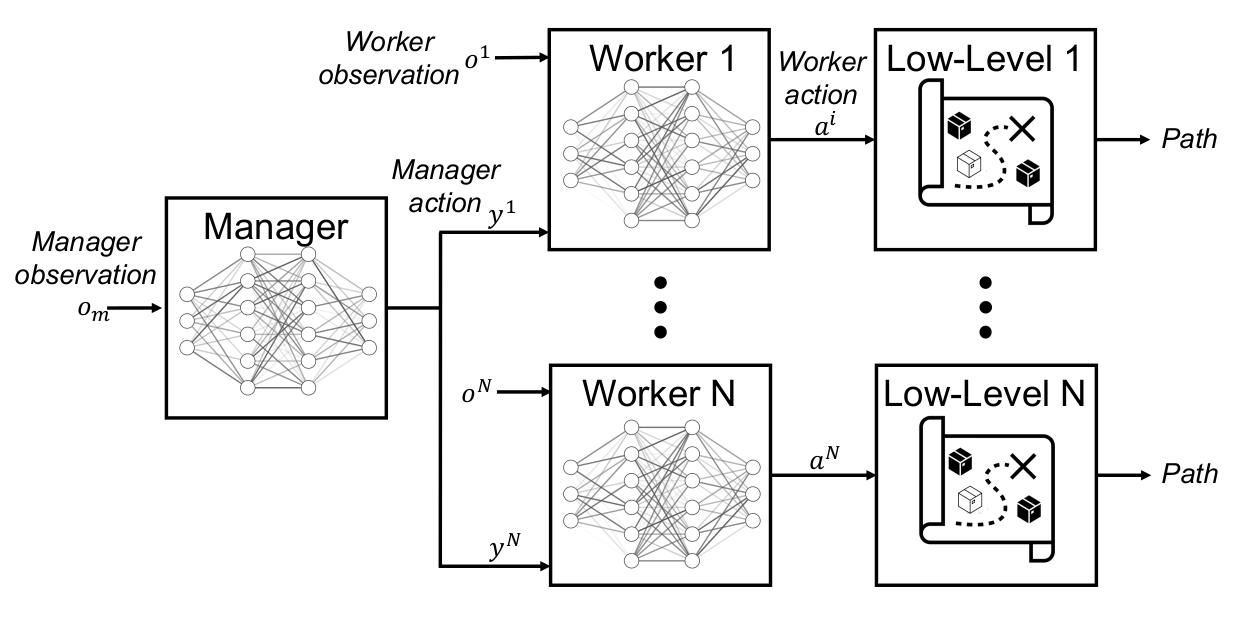
\includegraphics[width=0.65\textwidth]{hsnac-diagram.png}
    \caption{The Fedual Hierarchy architecture for the HSNAC MARL algorithm. \textit{(Image Credit: Krnjaic et al.)}}
    \label{fig:hsnac-dia}
\end{figure}


The warehouse simulator implemented with OpenAI gym interface was aimed to be scalable and computationally tractable with low 0.2 FPS (frames per second) i.e. 5 seconds passes in game world with each game episode step \cite{brockman2016openai}.
This low FPS degrades the performance with lower action frequency to some extent but simplifies model training with a reasonable enough time frame on which agent actions operate upon the environment.
For simplifications the collisions are not modeled in this environment, and the packages are also loaded automatically onto the AGVs without extra delays for additional quantity.
In the system spanning mechanism, the number of agents remains constant, workers don’t experience fatigue or failures, and the orders are assigned to AGVs in a first-in-first-out queue system.


In this formulation very uniquely agents select their task target location as their action rather than usual directional AGV navigation movements.
To supplement such actions, the Dijkstra’s algorithm shortest paths are cached in the table where warehouse locations are represented in the graph.
Significant memory resources are consumed for storing such path information, but it makes the path determination problem a hash-table lookup of \textit{O(1)}.
The distance calculations scales in complexity proportional to \textit{O($|$W$|$$|$L$|$)}, a KD-Tree for decomposing graph coordinate space and compiled vectorized function directly operation on machine was additionally used for optimality.


The MARL task interactions are formulated as POSG for N agents defined by seven dimensional tuple \cite{hansen2004dynamic}.
This tuple defines agent representations, state space, joint action space, partial observations, observation function, transition function, and reward function for all the agents in the system.
And, like any other RL problem the aim is to learn a joint policy for all agents that maximize the discounted reward returns.
The action space consists of mobile agents to visit all locations and pickers to visit all item locations.
This results in large action space and action is also dependent on the agent’s current and target locations.
For observations, both AGVs and pickers observe current and target location of other agents. But, only pickers observe complete order lists whereas the AGV observe only their current order.
Two different reward function schemes are followed for pickers and AGVs, where the picker is rewarded 0.1 for completing the pick at timestep \textit{t}, otherwise it is rewarded -0.05.
Second, for each AGV 0.1 reward is given when either picked item is received or order is completed at timestep \textit{t}, otherwise a reward of -0.05 is given.


\begin{figure}
\centering

\begin{subfigure}[b]{0.55\textwidth}
   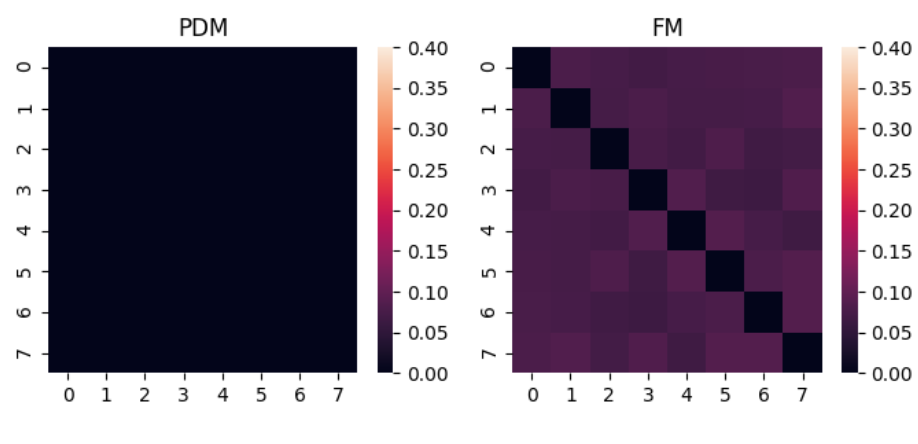
\includegraphics[width=1\linewidth]{pdm-fm.png}
   \caption{Warehouse zoning heatmaps for heuristic approaches PDM and FM respectively.}
   \label{fig:pdm-fm}
\end{subfigure}

\begin{subfigure}[b]{0.55\textwidth}
   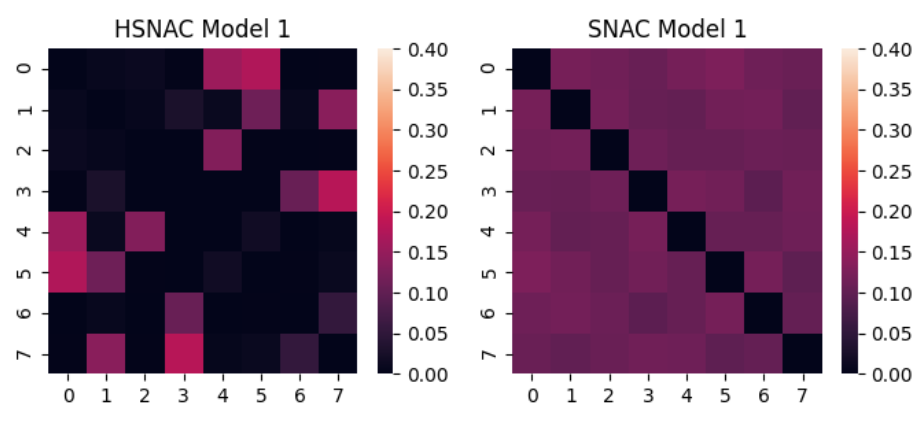
\includegraphics[width=1\linewidth]{hsnac-snac.png}
   \caption{Warehouse zoning heatmaps for MARL approaches HSNAC and SNAC respectively.}
   \label{fig:hsnac-snac} 
\end{subfigure}


\caption[Warehouse zoning heatmaps]{(a) Heatmaps for picker-to-picker order line completion similarity data for PDM and FM approaches. (b) Equivalent heatmaps highlighting similarity between HSNAC and PDM, and SNAC and FM approaches respectively. \textit{(Image Credit: Krnjaic et al.)}}
\end{figure}


The action space for each agent is really large, approximately being equal to the number of locations, and the actions will take different durations for terminations.
This study employs FMH where the manager produces goals for the subordinates as shown in Figure \ref{fig:hsnac-dia}.
This concept is used to partition warehouse locations into sectors, where managers observe current and target locations for the agents to guide agents into their sector locations.
After, the sector allocation agent’s policy selects the next target, and then lower level controllers calculate the path to execute a sequence of actions for reaching the target.
This sectoring strategy reduces the action space by a huge amount, and is further optimized by using action masking which filters out locations that are not part of the current order.
The proposed sector zoning and FMH model is trained with the Shared Network Actor-Critic (SNAC) architecture \cite{christianos2020shared}.
The policy and value component networks are represented by artificial neural networks (ANNs) having 128 input dimensions with ReLU activations, and outputs policy and value head for each agent.
Each agent is parametrized with critic and value component networks components having 64 input dimensions with ReLU outputs.


\subsubsection{Experiments and Results}


For scalable experimentation testing large warehouse configuration of 1276 locations, 16 AGVs, 8 pickers, 22 partitioned zones, and 80 orders which comprises 5 order-lines on average.
Also, pick rate in order-lines per hour was used as the primary performance measure for all the experimentation approaches.
It expresses average frequency picks per episode for trained HSNAC models in PyTorch for 8000 episodes and 8 seeds.
From Table \ref{table_scale_results}, it is observed that the HSNAC approach generally outperforms all other approaches except for FM benchmark approach.
This performance increase in pick rate is attributed to great reduction in idle time for AGVs and pickers but travel distance is increased to some extent.
Qualitatively, multiple pickers competed for AGVs in experimentation which demonstrates emergence of competitive behavior.
The approaches, PDM and FM utilize their pickers differently where PDM divides them in disjoint sectors, FM allows a more free movement.
Additionally, it was observed that for FM the lowest, and for HSNAC the second lowest episode length was observed.
A decrease in average episode length signifies efficient package delivery with reduced idle time.
From Figure \ref{fig:scale-learn-curve} it also demonstrated that HSNAC performs considerably well as compared to SNAC and PDM algorithms with higher pick rate throughput.


\begin{figure}[h]
    \centering
    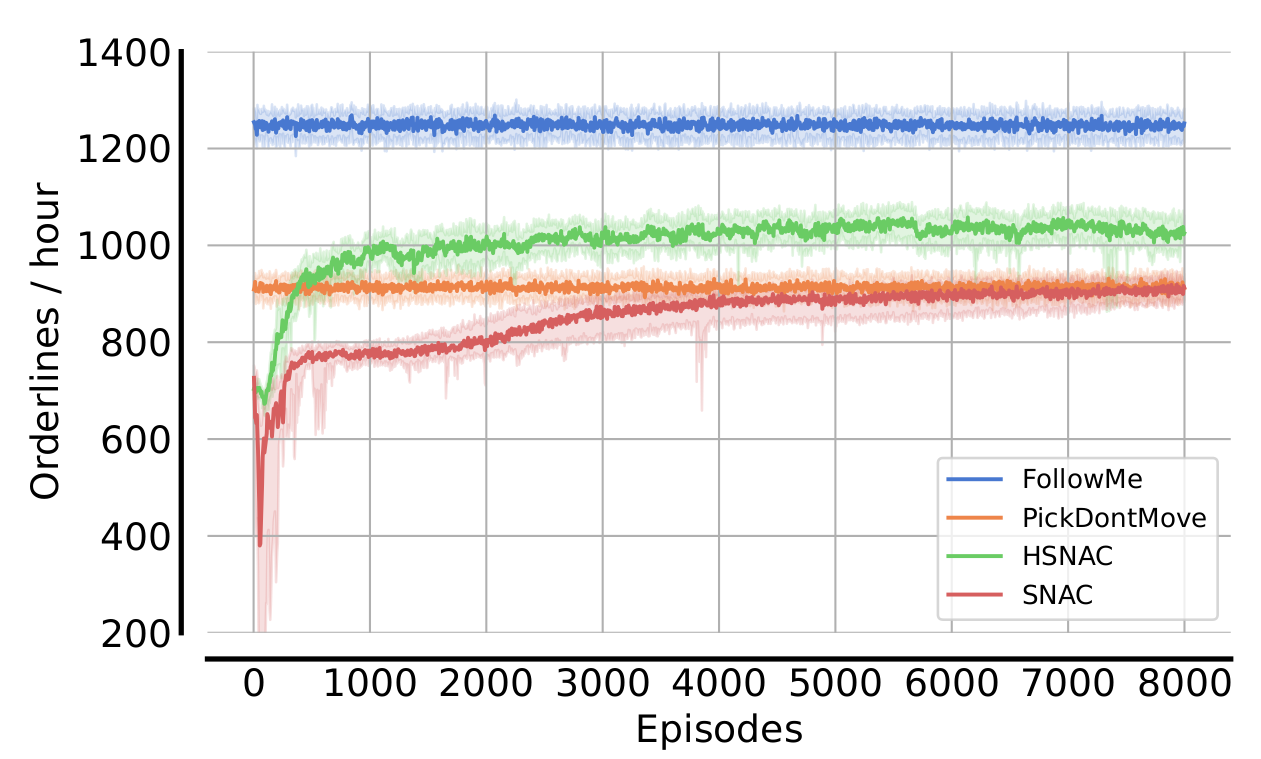
\includegraphics[width=0.6\textwidth]{rl-result-curve.png}
    \caption{System pipeline for the proposed scalable MARL solution. \textit{(Image Credit: Krnjaic et al.)}}
    \label{fig:scale-learn-curve}
\end{figure}


For measuring picker utilization of the benchmarked algorithms, the individual picker’s order-list completion location data is aggregated and normalized, and compared with cosine similarity measures of other pickers.
From Figure \ref{fig:pdm-fm}, we observe uniform similarity in FM, and no similarity with zoning strategy for PDM.
Similarly, with Figure \ref{fig:hsnac-snac} we observe some extent of zoning in HSNAC algorithm, and uniform cosine similarity in SNAC like FM approach.
It shows a structural emergence trend in the warehouse where picker regions seem to overlap with other pickers.
The main disadvantage of using FM approach is direct dependence on performance of pickers which can lead to throughput dropouts if picker productivity drops.
The major advantage of using HSNAC over the PDM industry standard is its flexibility i.e. it allows two or more pickers to serve secluded zones, and movement of pickers across zones as well.

\begin{table*}[t]
\centering
\caption{Performance metrics \textit{Distance(m)}, \textit{Idle Time(s)}, and \textit{Pick Rate} for HSNAC, SNAC, FM and PDM approaches with $\pm$95\% confidence interval for AGVs and pickers.}
     \label{table_scale_results}
    \begin{center}
        \begin{tabular}{ccccccc}
        \toprule
         \textbf{MARL}&\multicolumn{3}{c}{Metrics for AGVs}&\multicolumn{3}{c}{Metrics for Pickers}\\
         \textbf{Methods}&\textit{Distance}&\textit{Idle Time}&\textit{Pick Rate}&\textit{Distance}&\textit{Idle Time}&\textit{Pick Rate}\\
        \midrule 
        \textbf{HSNAC}&1887$\pm$3&779.48$\pm$1.91&69.99$\pm$0.10&2299$\pm$6&688.44$\pm$1.73&139.98$\pm$0.19\\
        {SNAC}&1975$\pm$3&952.57$\pm$2.10&63.80$\pm$0.08&3678$\pm$9&585.99$\pm$1.28&127.59$\pm$0.16\\
        \midrule 
        \midrule 
        \textbf{Heuristic}&\multicolumn{3}{c}{Metrics for AGVs}&\multicolumn{3}{c}{Metrics for Pickers}\\
         \textbf{Methods}&\textit{Distance}&\textit{Idle Time}&\textit{Pick Rate}&\textit{Distance}&\textit{Idle Time}&\textit{Pick Rate}\\
         \midrule 
        {PDM}&1529$\pm$4&1028.55$\pm$7.11&56.80$\pm$0.21&1104$\pm$5&1084.53$\pm$7.36&113.61$\pm$0.42\\
        \textbf{FM}&1970$\pm$5&514.13$\pm$2.33&78.78$\pm$0.25&1620$\pm$6&582.49$\pm$2.40&157.57$\pm$0.49\\
        \bottomrule
        \\
       \end{tabular}
     \end{center}
\end{table*}


\section{Discussion}


By exploring automated warehouse management approaches, for both heuristic and reinforcement learning paradigms we observe the high complexity associated with the task.
\footnote{Bibliography papers available at the repository \href{https://github.com/arana-initiatives/ai-portfolio-bibliography}{github.com/arana-initiatives/ai-portfolio-bibliography}.}
The heuristic approaches attempt to solve this problem as a modular problem, by optimizing each modular subproblem like TA and MAPF with traditional optimization and search based algorithms.
These approaches as we observe have less flexibility and require more engineering effort when the problem involves changing parameters and modules leading to shift in optimization goal.
Therefore, we further explore formulating this problem as MARL problem, which leads to different challenges from theoretical ones like reward shaping to more practical ones like scalability.
As part of this manuscript, we explored two studies which tackle these challenges and attempt to provide an end-to-end solution for the automated warehouse management problem.


% for dual reward shaping approach
% limitations: reward scheme not clear, stabalization in learning not visible, & finally initial reward value appears because reward being assigned for partial actions as well
% add the selection of mixed cooperation strategy usage here, 
% ameliorate the learning problem when the workload is concentrated on single agent ...
% division of reward requires domain knowledge for redistribution of reward signals
% issue the way action is defined, rather misleading
% reward shaping, does addtional reward actually stabalize learning or not,
% second the algorithm itself might not be effective while scaling
For its merit, the experimentation study with dual segmented reward shaping model achieves good performance with very simplistic RL algorithms with their approach.
But, still this study leaves out explanations of a plethora of experimentation factors in detail, and does not precisely quantify the performance gains.
First, the study mentions paradigms like, CTCE, CTDE etc. in their study but structurally does not explicitly give clarifications which paradigm their current approach belongs to or closely resembles.
More importantly, the environment does not support concepts of full or partial actions but rather granular actions that give 2D planar directions to agents.
Essentially meaning, that the reward model beholds more complexity which keeps track of subtask completion for each agent for reward distribution.
Or it transforms action space into these functionally high level subtask actions which reduces the problem complexity drastically in comparison to the initial sparse problem.
Additionally, these reward distribution magnitudes and their allocation are not discussed in precise detail in the study for each valid scenario.
As \textit{“move to”} partial actions relative sequence in Figures \ref{fig:reward-model-a} and \ref{fig:reward-model-b} matters, if \textit{“Move to Destination”} happens before \textit{“Move to Object”} the reward models will inconsistent.
For example, as per the reward model specified in Figure \ref{fig:reward-model-b} after taking \textit{“Move to Destination”} and \textit{“Return Tray”} actions the partial reward will get assigned to the agent even if the object is not delivered.
Hence, it is not made clear in the study whether the reward will only be assigned when specific complete reward sequences are traversed or partial reward with partial sequence will also be assigned.
Therefore, without valid implementation details or repository there are several ambiguities for determining the true efficacy of the results produced in this study.


Second, for validating results only convergence plots were used to measure the efficacy but average episode length for task completion would give a more complete picture of the true model performance and learning capabilities.
As agents in reward shaping agents are often vulnerable to fall for positive reward cycles, and it might be possible that agents are repeating sub subtasks.
This way agents are accumulating higher but redundant rewards which might not be necessary for the overall optimization process.
The reward model designed in the study does the majority of the heavy lifting in the learning task by breaking down the complex value function into a simpler value function alternative to learning with partial actions.
Also, this model might only be tuned for this particular type of package delivery design in the warehouse, and possibly will not generalize well with some changes in the problem.
Finally, the study does not compare its performance against other mentioned relevant approaches for sparse learning, like curiosity drive learning, curriculum learning etc.
The advantages listed for this study only operate on simpler scales with current architecture, and can be effective for small warehouses practically in fully automated settings. Also, the utilization of the reward model might help other state of the art methods (SOTA) to achieve better performance as well.


% for scalable learning approach
% high computational resources used, results section
% RL problem resembles closely the optmization one
The scalable hierarchical MARL study is highly scalable which is also compatible with existing real infrastructure and includes humans pickers as well.
This approach is rather more practical as including humans can reduce unexpected warehouse downtime in case of major robotic infrastructure failure.
Further, this approach unlike other MARL approaches defines very high level actions which lead agents directly to the location, which reduces the complexity drastically.
And, this formulation closely resembles heuristic approaches as with this MARL formulation the agents select the location path from their actions directly.
Unlike other standard MARL formulations the agent does not iteratively learn to explore in the environment with experience efficiently but rather learns to select the shortest path in the given scenario.
Storing such paths is a very computationally expensive step, and might introduce warehouse configuration consistency requirements, like heuristic approaches.
It is better than heuristic approaches from the aspect that order demand distribution does not affect the system performance.


With the FMH design for complexity reduction this study fails to surpass FM which utilizes its agents more effectively.
To its merit this study does outperform well established heuristic standard PDM, but with higher average travel distance which practically would cost higher robotic maintenance and human welfare concerns.
For realistic implementation the simplicity of the environment needs to be upgraded iteratively, as simulation results often cannot be directly translated to the real world applications \cite{zhao2020sim}.
For example, realistically loading may take variable time depending on the required quantity, the collision-free assumption would not hold in real world, requiring agents to re-route dynamically.
This study can further improve its results with addition of energy utilization penalization, and AGV agent communication to suppress the observed competitive behavior in the study.
Also, warehouses do not operate in isolation but are part of a bigger supply-chain infrastructure, and the proposed solution should be adaptive of these changes \cite{lu2018learning}.
Finally, the scalable solution provided in this study is very reasonable in terms of its MARL problem implementation and proposed enterprise design for deployment into the real world after the improvement suggestions.


\section{Conclusion}


In conclusion, with our exploration we observe the efficacy of using MARL approaches for the warehouse management problem, and increased flexibility for providing end-to-end pipeline with minimal use-case specific engineering efforts.
Second, we also explore different challenges associated with building scalable MARLS, and the engineering effort required for defining meaningful rewards for the same.
Further, the relevance of heuristic based methods is also demonstrated in the benchmarking scalable MARL study where the RL problem’s action space closely resembles heuristic problem formulation.
In our exploration, we couldn’t find the recent SOTA MARL methods being compared with the heuristic benchmarks for this task.
And, application of SOTA sparsity handling methodologies to mitigate the sparse rewards problem were also non-existent for this use-case.
Even after these existing literature and experimentation limitations, we observe that MARL problem formulation and system design are capable of building scalable and human-centric solutions for manufacturing sectors.


\bibliographystyle{acm}
\bibliography{main}


\end{document}

